\documentclass[12pt, titlepage]{article}

\usepackage{booktabs}
\usepackage{tabularx}
\usepackage{hyperref}
\usepackage{float}
\usepackage{graphicx}
\hypersetup{
    colorlinks,
    citecolor=blue,
    filecolor=black,
    linkcolor=red,
    urlcolor=blue
}
\usepackage[round]{natbib}

%% Comments

\usepackage{color}

\newif\ifcomments\commentstrue %displays comments
%\newif\ifcomments\commentsfalse %so that comments do not display

\ifcomments
\newcommand{\authornote}[3]{\textcolor{#1}{[#3 ---#2]}}
\newcommand{\todo}[1]{\textcolor{red}{[TODO: #1]}}
\else
\newcommand{\authornote}[3]{}
\newcommand{\todo}[1]{}
\fi

\newcommand{\wss}[1]{\authornote{blue}{SS}{#1}} 
\newcommand{\plt}[1]{\authornote{magenta}{TPLT}{#1}} %For explanation of the template
\newcommand{\an}[1]{\authornote{cyan}{Author}{#1}}

%% Common Parts

\newcommand{\progname}{Flick Picker}
\newcommand{\authname}{Team 7, 7eam
\\ Talha Asif - asift
\\ Jarrod Colwell - colwellj
\\ Madhi Nagarajan - nagarajm
\\ Andrew Carvalino - carvalia    
\\ Ali Tabar - sahraeia
}     

\usepackage{hyperref}
    \hypersetup{colorlinks=true, linkcolor=blue, citecolor=blue, filecolor=blue,
                urlcolor=blue, unicode=false}
    \urlstyle{same}
                                


\begin{document}

\title{System Verification and Validation Plan for \progname{}} 
\author{\authname}
\date{\today}
	
\maketitle

\pagenumbering{roman}

\section*{Revision History}
\begin{table}[hp]
	\caption{Revision History} \label{TblRevisionHistory}
	\begin{tabularx}{\textwidth}{llX}
		\toprule
		\textbf{Date} & \textbf{Developer(s)} & \textbf{Change}\\
		\midrule
		October 31 & Jarrod Colwell & Summary \& Objectives content added\\
		\midrule
		October 31 & Talha Asif & Added FR Tests\\
		\midrule
		November 1 & Ali Tabar & Added and formatted tests for Non-Functional Requirements\\
		\midrule
		November 1 & Ali Tabar & Filled in some tests for Non-Functional Requirements (Look and Feel T 1: Appearance, all of Performance)\\
		\midrule
		November 1 & Talha Asif & Filled Traceability Matrix\\
		\midrule
		November 2 & Andrew Carvalino & NFR tests\\
		\midrule
		November 2 & Madhi Nagarajan & Section 3\\
		\midrule
		November 2 & Jarrod Colwell & Final Edits\\
		\midrule
		April 5 & Andrew Carvalino & Added Survey to Appendix and made final edits\\
		\bottomrule
	\end{tabularx}
\end{table}


\newpage

\tableofcontents

\listoftables

\newpage

\section{Symbols, Abbreviations and Acronyms}

\renewcommand{\arraystretch}{1.2}
\begin{tabular}{l | l} 
  \toprule		
  \textbf{Symbol} & \textbf{Description}\\
  \midrule 
  T & Test\\
  V\&V & System Verification and Validation\\
  SRS & Software Requirements Specification\\
  UI & User Interface\\
  FR & Functional Requirement\\
  NFR & Non-Functional Requirement\\
  OAuth & Open Authorization\\
  \bottomrule
\end{tabular}\\

% \wss{symbols, abbreviations or acronyms -- you can simply reference the SRS \citep{SRS} tables, if appropriate}

\newpage

\pagenumbering{arabic}

This document contains the V\&{}V plan for Flick Picker, as well as the roadmap of when the tests will be implemented.

\section{General Information}

\subsection{Summary}
This document describes the plan to verify and validate that Flick Picker meets the defined requirements and specifications. Additionally, this document will validate that Flick Picker fulfills its intended purpose of recommending compatible Movies, TV Shows, or Anime to an individual or a group.

\subsubsection{Front End Testing}
\begin{itemize}
	\item Account Creation - Web page that facilitates user account creation
	\item User Preferences - Web page that facilitates user preference settings
	\item Group Creation - Web page that facilitates the creation of groups
	\item Recommendation - Web page that displays recommendations for an individual or group
\end{itemize}
\subsubsection{Back End Testing}
\begin{itemize}
	\item Database Access - Accessing the database to find user preferences or information pertaining to Movies, TV Shows, or Anime
	\item Recommendation Algorithm - The algorithm responsible for finding the best Movies, TV Shows, or Anime for an individual or group
	\item API Data - The accessing, storage, and usage of external data from various APIs
\end{itemize}

% \wss{Say what software is being tested.  Give its name and a brief overview of its general functions.}

\subsection{Objectives}
\subsubsection{Requirements}
The first objective involves verifying that Flick Picker meets requirements outlined in our SRS document and validating that the behaviour present is desirable. This includes the functional requirements (e.g. Authentication Requirements) and the non-functional requirements (e.g. Appearance Requirements). This objective will build confidence in the correctness of Flick Picker along with validating that security and usability standards are met.

\subsubsection{UI Elements}
The second objective of the V\&V document involves the validation of navigability and functionality of UI elements. Each menu described in the `Front End Testing' section above must be functional for users. Additionally, users must be able to navigate to each page individually. This objective ensures that usability and response time standards are met. 

\subsubsection{External Connections}
The final objective of the V\&V document is to ensure that all external connections of Flick Picker (e.g. APIs, Database) work as intended. This objective ensures that the interoperability of Flick Picker is adequate. 

%\wss{State what is intended to be accomplished.  The objective will be around the qualities that are most important for your project.  You might have something like: ``build confidence in the software correctness,'' ``demonstrate adequate usability.'' etc.  You won't list all of the qualities, just those that are most important.}

\subsection{Relevant Documentation}

% \wss{Reference relevant documentation.  This will definitely include your SRS and your other project documents (MG, MIS, etc). You can include these even before they are written, since by the time the project is done, they will be written.}
\begin{enumerate}
	\item[] SRS: \citet{SRS}
	\item[] MG: \citet{MG}
	\item[] MIS: \citet{MIS}
\end{enumerate}

\section{Plan}

Contains the plan for Flick Picker, going into detail about the team and verification plans

\subsection{Verification and Validation Team}
The Verification and Validation Team will consist of Internal (team) and External members.

\begin{enumerate}
	\item Team Members:
	\begin{enumerate}
		\item Ali: Ad-hoc or checklist verification of SRS, Design documents through peer-reviewing. Verification of implementation. For testing, responsible for creating/running frontend unit tests and system tests (Integration, Manual).
		\item Andrew: Ad-hoc or checklist verification of SRS, Design documents through peer-reviewing. Verification of implementation. For testing, responsible for creating/running frontend unit tests and system tests.
		\item Jarrod: Ad-hoc or checklist verification of SRS, Design documents through peer-reviewing. Verification of implementation. For testing, responsible for creating/running backend unit tests and system tests.
		\item Madhi: Ad-hoc or checklist verification of SRS, Design documents through peer-reviewing. Verification of implementation. For testing, responsible for creating/running frontend \& backend unit tests and system tests.
		\item Talha: Ad-hoc or checklist verification of SRS, Design documents through peer-reviewing. Verification of implementation. For testing, responsible for creating/running frontend \& backend unit tests and system tests.
	\end{enumerate}
	\item External Members
	\begin{enumerate}
		\item Classmates: Ad-hoc verification of SRS and Design documents.
		\item Course TAs and Instructors: Ad-hoc verification of SRS and Design documents. Ad-hoc verification of the app implementation.
		\item Users: Ad-hoc validation of application.
	\end{enumerate}
\end{enumerate}


\subsection{SRS Verification Plan}
For the SRS Verification Plan, an ad-hoc approach will be followed. Teammates will peer-review work done for the SRS to verify whether both the functional and non-functional requirements serve validity. The SRS checklist will be followed prior to the finalization of a revision by a team member. Classmates and instructors will ad-hoc review the Revision 0 of the SRS, again to verify the requirements.


\subsection{Design Verification Plan}
For the Design Verification Plan, an ad-hoc approach will be followed. Teammates will peer-review work done for the MG and MIS to verify whether both modules and their specification have validity. The MG and MIS checklists will be followed prior to the finalization of a revision by a team member. Classmates and instructors will ad-hoc review the Revision 0 of the MG and MIS, again to verify the modules.

\subsection{Implementation Verification Plan}
Our Implementation Verification Plan will mainly consist of system testing and unit testing, as specified in the latter sections of this document. These tests will ensure that our implementation meets the criteria for our functional and non-functional requirements.
Further means of implementation verification will also include code walkthroughs and reviews prior to pull request approvals. Static analysis and code coverage will also be incorporated to ensure that new code is written up-to standards. Verification tools will be explained in the latter sections.


\subsection{Automated Testing and Verification Tools}
Unit tests will be written with a JavaScript unit testing framework called Jest. Jest also produces reports for code coverage metrics. Our code coverage goals include an overall 80\% coverage. A code coverage check will be done for every Pull Request made. Code coverage reports will be monitored to ensure that all functionality is being tested. Integration/system tests will be done with Selenium and Cucumber.js. Cucumber.js also has functionality to produce testing metrics and results. For static analysis and linting, ESLint and AirBnB styling will be utilized. This will ensure uniform coding standards and uncover any potential errors prior to compilation. Auomated code builds, through GitHub/Jenkins, will be present to ensure that every deployment made will not break the application. Refer to Development Plan for indepth details behind the tools:

\citet{DevPlan}


\subsection{Software Validation Plan}
For software validation, our team will host review sessions with target users of our application. During this session, these users will interact with the application and we will record their experiences. Based on the data collected, it will allow us to validate whether our requirements fulfills the goal of our application.

\section{System Test Description}
The tests outlined here will follow the following format:
\paragraph*{Test \#{}: Test Title}
\begin{itemize}
	\item[Control:] FR: Manual or Automated | NFR: Functional, Dynamic, Manual, or Static
	\item[Initial State:] Initial State
	\item[Input:] Input
	\item[Output:] Output
	\item[Derivation:] Test Case Derivation
	\item[Execution:] Manual Test | API Test
\end{itemize}
The execution of the test will be through automated selenium tests for the front-end and an API test library for the back-end.

\subsection{Tests for Functional Requirements}
The tests below are based directly on the FR sections from the SRS. Since these are mandatory requirements, they will all be automated, and the tests must pass on any new code change to prevent these requirements from being violated.

\subsubsection{Area of Testing: Authentication}
Contains all the tests for the Authentication FR.

\paragraph*{UI Auth T 1: User Login - Success}
\begin{itemize}
	\item[Control:] Automated
	\item[Initial State:] Empty email and password box, on the login screen. Pre-existing test customer exists.
	\item[Input:] Email and password is filled correctly
	\item[Output:] Customer is logged in
	\item[Derivation:] Need a successful UI test on what a customer will see once they are logged in correctly
	\item[Execution:] Manual Test
\end{itemize}

\paragraph*{API Auth T 1: User Login - Success}
\begin{itemize}
	\item[Control:] Automated
	\item[Initial State:] Pre-existing test customer exists.
	\item[Input:] `login' API is targeted with correct credentials filled in
	\item[Output:] Success response is returned (200)
	\item[Derivation:] Need a successful API test on how the login API will respond to correct information
	\item[Execution:] API Test
\end{itemize}

\paragraph*{UI Auth T 2: User Login - Failure}
\begin{itemize}
	\item[Control:] Automated
	\item[Initial State:] Empty email and password box, on the login screen. Pre-existing test customer exists.
	\item[Input:] Email and password is filled incorrectly
	\item[Output:] Customer failed to login
	\item[Derivation:] Need a successful failure UI test on what a customer will see once they input their credentials incorrectly
	\item[Execution:] Manual Test
\end{itemize}

\paragraph*{API Auth T 2: User Login - Failure}
\begin{itemize}
	\item[Control:] Automated
	\item[Initial State:] Pre-existing test customer exists.
	\item[Input:] `login' API is targeted with incorrect credentials filled in
	\item[Output:] Failure response is returned (401)
	\item[Derivation:] Need a successful API test on how the login API will respond to incorrect information
	\item[Execution:] API Test
\end{itemize}

\paragraph*{UI Auth T 3: User Sign-Up - Success}
\begin{itemize}
	\item[Control:] Automated
	\item[Initial State:] Empty email and password box, on the login screen.
	\item[Input:] Sign-up button is pressed, all boxes for sign-up are filled in correctly, confirm button is pressed
	\item[Output:] Customer account is created
	\item[Derivation:] Need a successful UI test on what a customer will see once they Sign-Up correctly
	\item[Execution:] Manual Test
\end{itemize}

\paragraph*{API Auth T 3: User Sign-Up - Success}
\begin{itemize}
	\item[Control:] Automated
	\item[Initial State:] Not Applicable
	\item[Input:] `signup' API is targeted with information correctly filled in
	\item[Output:] Success response is returned (200) and customer account is created
	\item[Derivation:] Need a successful API test on how the signup API will respond to correct information
	\item[Execution:] API Test
\end{itemize}

\paragraph*{UI Auth T 4: User Sign-Up - Failure}
\begin{itemize}
	\item[Control:] Automated
	\item[Initial State:] Empty email and password box, on the login screen.
	\item[Input:] Sign-up button is pressed, all boxes for sign-up are filled in incorrectly, confirm button is pressed
	\item[Output:] Areas where there is incorrect information is highlighted
	\item[Derivation:] Need a successful UI test on what a customer will see if they do not Sign-Up correctly
	\item[Execution:] Manual Test
\end{itemize}

\paragraph*{API Auth T 4: User Sign-Up - Failure}
\begin{itemize}
	\item[Control:] Automated
	\item[Initial State:] Not Applicable
	\item[Input:] `signup' API is targeted with information incorrectly filled in
	\item[Output:] Failure response is returned (422) and customer account is not created
	\item[Derivation:] Need a successful API test on how the signup API will respond to correct information
	\item[Execution:] API Test
\end{itemize}

\paragraph*{UI Auth T 5: User Logout}
\begin{itemize}
	\item[Control:] Automated
	\item[Initial State:] Test customer is logged in, on home page
	\item[Input:] Logout is pressed
	\item[Output:] Login screen displays
	\item[Derivation:] Need a UI test on what a customer will see if they log out
	\item[Execution:] Manual Test
\end{itemize}

\paragraph*{API Auth T 5: User Logout}
\begin{itemize}
	\item[Control:] Automated
	\item[Initial State:] Test customer is logged in
	\item[Input:] `logout' API is targeted with the test customer information
	\item[Output:] Success response is returned (500)
	\item[Derivation:] Need to test the logout API
	\item[Execution:] API Test
\end{itemize}

\paragraph*{UI Auth T 6: User OAuth Sign-Up/Login}
\begin{itemize}
	\item[Control:] Automated
	\item[Initial State:] Empty email and password box, on the login screen.
	\item[Input:] OAuth button is pressed
	\item[Output:] Correctly redirect to OAuth login
	\item[Derivation:] Need a successful UI test on what a customer will see if they choose to sign-up/login though an OAuth provider
	\item[Execution:] Manual Test
\end{itemize}

\subsubsection{Area of Testing: Profile/Group}
Contains all the tests for the Profile/Group FRs.

\paragraph*{UI PG T 1: Modify User Profile}
\begin{itemize}
	\item[Control:] Automated
	\item[Initial State:] On home page
	\item[Input:] Profile button is clicked, display name and password are updated, confirm is clicked
	\item[Output:] Confirmation that information is updated
	\item[Derivation:] Need a successful UI test on how a customer can update their profile
	\item[Execution:] Manual Test
\end{itemize}

\paragraph*{API PG T 1: Modify User Profile}
\begin{itemize}
	\item[Control:] Automated
	\item[Initial State:] Not Applicable
	\item[Input:] `updateProfile' API is targeted with data to update
	\item[Output:] Success status is returned (200)
	\item[Derivation:] Need a successful API test on how a customer can update their profile
	\item[Execution:] API Test
\end{itemize}

\paragraph*{UI PG T 2: Modify User Preferences}
\begin{itemize}
	\item[Control:] Automated
	\item[Initial State:] On home page
	\item[Input:] Profile button is clicked, show preferences are updated, confirm is clicked
	\item[Output:] Confirmation that preferences are updated
	\item[Derivation:] Need a successful UI test on how a customer can update their preferences
	\item[Execution:] Manual Test
\end{itemize}

\paragraph*{API PG T 2: Modify User Preferences}
\begin{itemize}
	\item[Control:] Automated
	\item[Initial State:] Not Applicable
	\item[Input:] `updatePreferences' API is targeted with data to update
	\item[Output:] Success status is returned (200)
	\item[Derivation:] Need a successful API test on how a customer can update their preferences
	\item[Execution:] API Test
\end{itemize}

\paragraph*{UI PG T 3: Create Group}
\begin{itemize}
	\item[Control:] Automated
	\item[Initial State:] On home page
	\item[Input:] Create Group button is clicked, name is input, confirm is clicked
	\item[Output:] Group is created with the specified name
	\item[Derivation:] Need a successful UI test on how a customer can create a group
	\item[Execution:] Manual Test
\end{itemize}

\paragraph*{API PG T 3: Create Group}
\begin{itemize}
	\item[Control:] Automated
	\item[Initial State:] Not Applicable
	\item[Input:] `createGroup' API is targeted with name specified
	\item[Output:] Success status is returned (200) and group is created
	\item[Derivation:] Need a successful API test on how a customer can create a group
	\item[Execution:] API Test
\end{itemize}

\paragraph*{UI PG T 4: Join Group}
\begin{itemize}
	\item[Control:] Automated
	\item[Initial State:] On home page
	\item[Input:] Invite is accepted through notifications
	\item[Output:] User is added to the group
	\item[Derivation:] Need a successful UI test on how a customer can join a group
	\item[Execution:] Manual Test
\end{itemize}

\paragraph*{API PG T 4: Join Group}
\begin{itemize}
	\item[Control:] Automated
	\item[Initial State:] Not Applicable
	\item[Input:] `acceptInvite' API is targeted
	\item[Output:] Success response is returned (200)
	\item[Derivation:] Need a successful API test on how a customer can join a group
	\item[Execution:] API Test
\end{itemize}

\paragraph*{UI PG T 5: Invite to Group}
\begin{itemize}
	\item[Control:] Automated
	\item[Initial State:] On home page
	\item[Input:] Group is selected, invite user through their username or email, confirm is clicked
	\item[Output:] User invite is sent
	\item[Derivation:] Need a successful UI test on how a customer can send an invite
	\item[Execution:] Manual Test
\end{itemize}

\paragraph*{API PG T 5: Invite to Group}
\begin{itemize}
	\item[Control:] Automated
	\item[Initial State:] Not Applicable
	\item[Input:] `sendInvite' API is targeted
	\item[Output:] Success response is returned (200)
	\item[Derivation:] Need a successful API test on how a customer can send an invite
	\item[Execution:] API Test
\end{itemize}

\subsubsection{Area of Testing: Recommendation}
Contains all the tests for the Recommendation FRs.

\paragraph*{UI R T 1: Receive Recommendations}
\begin{itemize}
	\item[Control:] Automated
	\item[Initial State:] On home page
	\item[Input:] Not Applicable
	\item[Output:] Observe if the home page is updated with recommendations
	\item[Derivation:] Need a successful UI test where a customer gets rotating recommendations
	\item[Execution:] Manual Test
\end{itemize}

\paragraph*{API R T 1: Receive Recommendations}
\begin{itemize}
	\item[Control:] Automated
	\item[Initial State:] Not Applicable
	\item[Input:] `viewRecommendations' API is targeted
	\item[Output:] Success response is returned (200) along with the list of shows
	\item[Derivation:] Need a successful API test where a customer gets rotating recommendations
	\item[Execution:] API Test
\end{itemize}

\paragraph*{UI R T 2: Rate Recommendations}
\begin{itemize}
	\item[Control:] Automated
	\item[Initial State:] On home page
	\item[Input:] Hover a movie and input recommendation
	\item[Output:] Movie should be updated with the recommendation
	\item[Derivation:] Need a successful UI test where a customer can update recommendations
	\item[Execution:] Manual Test
\end{itemize}

\paragraph*{API R T 2: Rate Recommendations}
\begin{itemize}
	\item[Control:] Automated
	\item[Initial State:] Not Applicable
	\item[Input:] `rateRecommendations' API is targeted along with enum data type
	\item[Output:] Success response is returned (200) and the movie recommendation is stored
	\item[Derivation:] Need a successful API test where a customer gets updated recommendations
	\item[Execution:] API Test
\end{itemize}

\paragraph*{API R T 3: Recommendation Match}
\begin{itemize}
	\item[Control:] Automated
	\item[Initial State:] Not Applicable
	\item[Input:] `findSharedRecommendation' API is targeted along with 5 user preferences
	\item[Output:] Success response is returned (200) and a show is selected with shared preferences
	\item[Derivation:] Need a successful API test where a group gets a recommended show
	\item[Execution:] API Test
\end{itemize}

\paragraph*{API R T 4: Recommendation Mismatch}
\begin{itemize}
	\item[Control:] Automated
	\item[Initial State:] Not Applicable
	\item[Input:] `findSharedRecommendation' API is targeted along with 5 user preferences, with entirely different preferences
	\item[Output:] Success response is returned (200) and a show is selected with shared the highest number of shared preferences
	\item[Derivation:] Need a successful API test where a group gets a recommended show where none of their preferences matched
	\item[Execution:] API Test
\end{itemize}

\subsection{Tests for Nonfunctional Requirements}

The tests below are based directly on the NFR sections from the SRS. Not all tests will be automated due to the nature of the requirement being tested.
We have also deemed to not test Scalability, due to the nature of that requirement.

\subsubsection{Area of Testing: Look and Feel}

Contains all the tests for the Look and Feel NFR.

\paragraph*{Look and Feel T 1: Appearance}
\begin{itemize}
	\item[Control:] Manual
	\item[Initial State:] Empty email and password box on the login screen
	\item[Input:] Any and all appropriate user inputs and navigation (typing login info, clicking buttons)
	\item[Output:] Visiting all menus and triggering all possible UI changes
	\item[Derivation:] Program's visual look in the real world (proper buttons / menus appearing, alignment, etc) should be approved by a real user
	\item[Execution:] Manual User Test
\end{itemize}

\paragraph*{Look and Feel T 2: Ease of Use}
\begin{itemize}
	\item[Control:] Non-Functional
	\item[Initial State:] System is in the login screen state
	\item[Input:] User logs in and explores the different screens and services offered
	\item[Output:] User goes through the system and provide feedback on the style choices (such as size of buttons or overall colour palette)
	\item[Derivation:] The test is meant to assess how different users may feel about style decisions and offer feedback on what looks and feels good to them and what needs improvement
	\item[Execution:] Survey
\end{itemize}

\subsubsection{Area of Testing: Usability and Humanity Tests}

\paragraph*{Usability and Humanity T 1: Ease of Use}
\begin{itemize}
	\item[Control:] Non-Functional
	\item[Initial State:] System is in the login screen state
	\item[Input:] User logs in and explores the different screens and services offered
	\item[Output:] User goes through the system without needing to ask for assistence or misunderstanding the affordances of the different screens
	\item[Derivation:] The test case is meant to assess whether the presentation of the system informs users of different technological skill levels of what functionality is provided by whatever state/screen they may be on
	\item[Execution:] User Test
\end{itemize}

\paragraph*{Usability and Humanity T 2: Learning}
\begin{itemize}
	\item[Control:] Non-Functional
	\item[Initial State:] Users have just finished Test \#3
	\item[Input:] Users are given a survey of how easy/complicated their experience using the system was
	\item[Output:] The surveys are filled out and collected
	\item[Derivation:] This survey is a continuation of Test \#3, with its results providing feedback as to whether the GUI of the system is understandable to users of different skill levels
	\item[Execution:] Survey
\end{itemize}

\subsubsection{Area of Testing: Performance}

Contains all the tests for the Performance NFR.

\paragraph*{Performance T 1: User Input Responsiveness}
\begin{itemize}
	\item[Control:] Dynamic
	\item[Initial State:] Any menu
	\item[Input:] Any user input (entering text, clicking a button)
	\item[Output:] Appropriate program response to user input
	\item[Derivation:] Must time the responsiveness of the program to an arbitrary user action in order to gauge if it is below 1 second.
	\item[Execution:] Manual Test
\end{itemize}

\paragraph*{Performance T 2: Safety-Critical}
\begin{itemize}
	\item[Control:] Dynamic
	\item[Initial State:] Empty email and password box on the login screen
	\item[Input:] Any and all appropriate user inputs and navigation (typing login info, clicking buttons)
	\item[Output:] Visiting all menus and triggering all possible UI changes, verifying with Selenium that no user information is outputted on the page
	\item[Derivation:] Ensuring that the application handles the user's private data properly and does not output it due to any unforeseen condition
	\item[Execution:] Manual Test
\end{itemize}

\paragraph*{Performance T 3: Precision or Accuracy}
\begin{itemize}
	\item[Control:] Manual
	\item[Initial State:] Main screen to generate a recommended media match for a previously created and inputted group
	\item[Input:] Clicking the button to generate the match
	\item[Output:] The media match
	\item[Derivation:] Must assess accuracy of program's ability to find something that everyone in the group should enjoy
	\item[Execution:] Conduct a survey using a fixed amount of people, and have each of them create an account. An effort should be made to choose a group of respondents that have a wide variety of preferences for the different categories of media available on Flick Picker. They will create and join multiple groups among each other using the application, and search for matches in each of these distinct groups. The survey will inquire respondents about each group, and how accurate they perceive their matches were each given group.
\end{itemize}

\paragraph*{Performance T 4: Reliability and Availability}
\begin{itemize}
	\item[Control:] Dynamic
	\item[Initial State:] Online application with server running
	\item[Input:] Visiting the web page
	\item[Output:] Connection success or failure
	\item[Derivation:] Checking to see if the web application is available for at least 90\% of the day, assuming Firebase stability
	\item[Execution:] Manual Test
\end{itemize}

\paragraph*{Performance T 5: Robustness or Fault-Tolerance}
\begin{itemize}
	\item[Control:] Dynamic
	\item[Initial State:] Main screen to generate a recommended media match for a previously created and inputted group. This group will be comprised of unique and few preferences.
	\item[Input:] Input
	\item[Output:] Output
	\item[Derivation:] Verifying that a match will always be found by stress testing using some heterogeneous groups
	\item[Execution:] Manual Test
\end{itemize}

\paragraph*{Performance T 6: Capacity}
\begin{itemize}
	\item[Control:] Dynamic
	\item[Initial State:] 0 users logged on the application
	\item[Input:] Several users logging onto the application
	\item[Output:] Application's stability
	\item[Derivation:] Ensuring and proving that each user session is independent of another and that no
	limit to the number of users logged on concurrently exists.
	\item[Execution:] Manual Test
\end{itemize}

\subsubsection{Area of Testing: Operational and Environmental Test}

\paragraph*{Operational and Environmental T 1: Interfacing with Adjacent Systems}
\begin{itemize}
	\item[Control:] Manual
	\item[Initial State:] System is in the login menu state
	\item[Input:] Developer will use the system as a regular user would on different web browsers
	\item[Output:] The system will have the same fundamental functionalities on all browsers, with perhaps minor differences in visual presentation
	\item[Derivation:] Developer will go through the various functionalities of the system on different web browsers, such as Chrome and Firefox, to assess whether or not it works and is usable on each
	\item[Execution:] Developer Exploration Test
\end{itemize}

\subsubsection{Area of Testing: Maintainability and Support Tests}

\paragraph*{Maintainability and Support T 1: Adaptability}
\begin{itemize}
	\item[Control:] Manual
	\item[Initial State:] System is in the login menu state
	\item[Input:] Developer will use the system as a regular user would on different mobile devices
	\item[Output:] The system will have the same fundamental functionalities on different mobile devices, with perhaps minor differences in visual presentation
	\item[Derivation:] Developer will go through the various functionalities of the system to assess whether or not it works and is usable on each
	\item[Execution:] Developer Exploration Test
\end{itemize}

\subsubsection{Area of Testing: Security Tests}

\paragraph*{Security T 1: Access}
\begin{itemize}
	\item[Control:] Manual
	\item[Initial State:] System is in the main menu state
	\item[Input:] Developer will click on their user profile and test the ability to change settings, as well as view the profile information of other users and ensure they cannot change their settings
	\item[Output:] The Developer's user profile will be changed, with such changes being visible to other users (if the setting was one which can be viewed by others) with the content of other profiles being unchangeable
	\item[Derivation:] Developer will ensure that the user's data is changable, that changes to public information can be viewed by others, that others' settings cannot be changed, and private information cannot be viewed by other users
	\item[Execution:] Developer Exploration Test
\end{itemize}

\paragraph*{Security T 2: Integrity}

\begin{itemize}
	\item[Control:] Manual
	\item[Initial State:] System is in the main menu state
	\item[Input:] Developer will change a profile or preference setting
	\item[Output:] After different increments of time after the changes are made (such as immediately, 1 hour, and 24 hours after) the Developer will verify that all the changes made persist and do not revert to a prior state
	\item[Derivation:] This is the best way to verify that information persists and retains its integrity over time, with it being possible to infer future persistence of information after the testing period
	\item[Execution:] Developer Exploration Test
\end{itemize}

\subsection{Traceability Between Test Cases and Requirements}

The two traceability matrices can be found in the Appendix.

\section{Unit Test Description}

%\wss{Reference your MIS and explain your overall philosophy for test case
%  selection.}
%\wss{This section should not be filled in until after the MIS has
%  been completed.}
%
In creating unit tests, we wanted to prioritize those functions of the system that were most important in order that it may work. 
This meant creating tests that covered the essentials and, in some cases, could be mapped onto similar functions (such as the group voting session testing 
results being applicable to individual voting, thereby eliminating the need to test the latter). Tests whose results followed from those of others were not 
included for the sake of brevity.

\subsection{Unit Testing Scope}
%
%\wss{What modules are outside of the scope.  If there are modules that are
%  developed by someone else, then you would say here if you aren't planning on
%  verifying them.  There may also be modules that are part of your software, but
%  have a lower priority for verification than others.  If this is the case,
%  explain your rationale for the ranking of module importance.}
%
M3, M5, M6, and M8 is the scope of the modules tested with unit testing. Each of these modules had functions that were vital to the 
system as a whole, and so they were prioritized for unit testing to speed up the testing process whenever large updates to the source code were made. 
We chose to leave out M4 (the Friends Module) since the creation of new test users and adding them as friends was a feature that could easily be verified 
manually and, if something was wrong with it, would be covered by the tests for the Groups Module. Similarly, M9 (OAuth Module) was left out of the scope 
since its functionality relied on what is provided by Google and Meta. Finally, M10 (API Module) was also left out of the scope since it, too, was dependent 
on what is provided by the API developers.


\subsection{Tests for Functional Requirements}
%
%\wss{Most of the verification will be through automated unit testing.  If
%  appropriate specific modules can be verified by a non-testing based
%  technique.  That can also be documented in this section.}
%
\subsubsection{Module 3 - Native Login}
%
%\wss{Include a blurb here to explain why the subsections below cover the module.
%  References to the MIS would be good.  You will want tests from a black box
%  perspective and from a white box perspective.  Explain to the reader how the
%  tests were selected.}
%
The most important function of this module is the creation of new accounts, with their data being uploaded to the database, thereby making 
the functionality of logging in inferrable from the success of this unit test.

\begin{enumerate}

\item[]{T1: User Creation\\}

Type: Automatic

Initial State: Login Page

Input: Test email and password

Output: New user profile created and added to database

Test Case Derivation: Ensure that the user creation funcationality works

How test will be performed: automatic testing file (user.test.ts)

\end{enumerate}

\subsubsection{Module 5 - Groups}

The funcationality of the Groups Module was fully covered by testing the creation of a group and all funcationality surrounding the adding of new members.

\begin{enumerate}

\item[]{T2: Create a group\\}

Type: Automatic

Initial State: Create Group Page

Input: Test group name

Output: New group is created

Test Case Derivation: Ensure that users can successfully create new groups

How test will be performed: automatic testing file (group.test.ts)

\item[]{T3: Add user to group\\}

Type: Automatic

Initial State: Social Page

Input: Group name and user id/email

Output: varification that selected user has been added to group

Test Case Derivation: Ensure that users can successfully be added to groups

How test will be performed: automatic testing file (group.test.ts)

\item[]{T4: Invite a user to group\\}

Type: Automatic

Initial State: Social Page

Input: Group name and friend id/email

Output: New user recieves invite to test group

Test Case Derivation: Ensure that users can successfully invite new members to groups

How test will be performed: automatic testing file (group.test.ts)

\item[]{T5: Accept Invite to group\\}

Type: Automatic

Initial State: Join Group Page

Input: Group invite id

Output: User accepts the group invite

Test Case Derivation: Ensure that users can successfully accept invitations to new groups

How test will be performed: automatic testing file (group.test.ts)

\end{enumerate}

\subsubsection{Module 6 - Profile}
%
%\wss{Include a blurb here to explain why the subsections below cover the module.
%  References to the MIS would be good.  You will want tests from a black box
%  perspective and from a white box perspective.  Explain to the reader how the
%  tests were selected.}
%
The changes to the profile section all used similar functionality with Firebase, so we thought it only necessary to test the creation of a 
new username. Moreover, the preferenes were fully tested, with initial and later preference changes being accounted for.
\begin{enumerate}

\item[]{T6: Edit user profile\\}

Type: Automatic

Initial State: Change User Name Page

Input: New user profile name

Output: Newly entered profile name is saved and displays instead of email or previous profile name

Test Case Derivation: Ensure that the user can successfully change their profile name

How test will be performed: automatic testing file (user.test.ts)

\item[]{T7: New preferences for a user\\}

Type: Automatic

Initial State: Preferences Page

Input: Set of media preferences

Output: Creation of the user's first set of preferences

Test Case Derivation: Ensure that the user can successfully create their initial preferences

How test will be performed: automatic testing file (user.test.ts)

\item[]{T8: Edit user preferences\\}

Type: Automatic

Initial State: Preferences Page

Input: Set of media preferences

Output: Change the user's first set of preferences to the newly specified preferences

Test Case Derivation: Ensure that the user can successfully change their preferences

How test will be performed: automatic testing file (user.test.ts)

\end{enumerate}

\subsubsection{Module 8 - Matching Algorithm}

The matching algorithm was fully tested, with the voting session, recommendations, votes, and final suggestion all being accounted for.

\begin{enumerate}

\item[]{T9: Start a Voting Session\\}

Type: Automatic

Initial State: Group Page

Input: Group id

Output: New voting session for test group

Test Case Derivation: Ensure that the group can start a new voting session

How test will be performed: automatic testing file (recommendation.test.ts)

\item[]{T10: Load Recommendations\\}

Type: Automatic

Initial State: Group Voting Page

Input: Group and session id

Output: Recommendations for the group

Test Case Derivation: Ensure that the algorithm can generate recommendations based on the preferences of all members

How test will be performed: automatic testing file (recommendation.test.ts)

\item[]{T11: Submit Votes\\}

Type: Automatic

Initial State: Group Voting Page

Input: Session id and votes for suggested media

Output: Verification that the users' votes are saved

Test Case Derivation: Ensure that the system can save users' votes for different media

How test will be performed: automatic testing file (recommendation.test.ts)

\item[]{T12: Find Best Match\\}

Type: Automatic

Initial State: Group Voting Page

Input: Session id

Output: The media that the algorithm chooses based on preferences and votes

Test Case Derivation: Ensure that the algorithm can provide a decision based on the suggestions and votes

How test will be performed: automatic testing file (recommendation.test.ts)

\end{enumerate}

%
\subsection{Tests for Nonfunctional Requirements}
There were no nonfunctional unit tests, as all nonfunctional requirements were tested through different means (such as the survey, as seen in the Appendix).

%
%\wss{If there is a module that needs to be independently assessed for
%  performance, those test cases can go here.  In some projects, planning for
%  nonfunctional tests of units will not be that relevant.}
%
%\wss{These tests may involve collecting performance data from previously
%  mentioned functional tests.}

%
\subsection{Traceability Between Test Cases and Modules}
%
%\wss{Provide evidence that all of the modules have been considered.}
\begin{table}[H]
	\caption{Module Traceability Matrix}
	\begin{tabular}{ll}
		\toprule
		\textbf{Test Number} & \textbf{Module} \\
		\midrule
		T1: User Creation & M3\\
		T2: Create a group & M5\\
		T3: Add user to group & M5\\
		T4: Invite a user to group & M5\\
		T6: Edit user profile & M6\\
		T7: New preferences for a user & M6\\
		T8: Edit user preferences & M6\\
		T9: Start a Voting Session & M8\\
		T10: Load Recommendations & M8\\
		T11: Submit Votes & M8\\
		T12: Find Best Match & M8\\
		\bottomrule
	\end{tabular}
\end{table}

\newpage

\bibliographystyle{plainnat}
\bibliography{../../refs/References}

\newpage

\section*{Appendix}

\begin{table}[H]
	\caption{Traceability Matrix 1} \label{TraceMatrix1}
	\begin{tabular}{ll}
		\toprule
		\textbf{Test Number} & \textbf{Requirement} \\
		\midrule
		UI Auth T 1 & FR 1\\
		API Auth T 1 & FR 1\\
		UI Auth T 2 & FR 1\\
		API Auth T 2 & FR 1\\
		UI Auth T 3 & FR 1\\
		API Auth T 3 & FR 1\\
		UI Auth T 4 & FR 1\\
		API Auth T 4 & FR 1\\
		UI Auth T 5 & FR 3\\
		API Auth T 5 & FR 3\\
		UI Auth T 6 & FR 2\\
		\midrule
		UI PG T 1 & FR 4\\
		API PG T 1 & FR 4\\
		UI PG T 2 & FR 5\\
		API PG T 2 & FR 5\\
		UI PG T 3 & FR 6\\
		API PG T 3 & FR 6\\
		UI PG T 4 & FR 7\\
		API PG T 4 & FR 7\\
		UI PG T 5 & FR 8\\
		API PG T 5 & FR 8\\
		\midrule
		UI R T 1 & FR 9\\
		API R T 1 & FR 9\\
		UI R T 2 & FR 10\\
		API R T 2 & FR 10\\
		UI R T 3 & FR 11\\
		API R T 3 & FR 11\\
		\bottomrule
	\end{tabular}
\end{table}

\begin{table}[H]
	\caption{Traceability Matrix 2} \label{TraceMatrix2}
	\begin{tabular}{ll}
		\toprule
		\textbf{Test Number} & \textbf{Requirement} \\
		\midrule
		Look and Feel T 1 & 10.1.1\\
		Look and Feel T 2 & 10.1.2\\
		\midrule
		Usability and Humanity T 1 & 10.2.1\\
		Usability and Humanity T 2 & 10.2.3\\
		\midrule
		Performance T 1 & 10.3.1\\
		Performance T 2 & 10.3.2\\
		Performance T 3 & 10.3.3\\
		Performance T 4 & 10.3.4\\
		Performance T 5 & 10.3.5\\
		Performance T 6 & 10.3.6\\
		\midrule
		Operational and Environmental T 1 & 10.4.3\\
		\midrule
		Maintainability and Support T 1 & 10.5.3\\
		\midrule
		Security T 1 & 10.6.1\\
		Security T 2 & 10.6.2\\
		\bottomrule
	\end{tabular}
\end{table}

\newpage

\subsubsection*{User Survey}
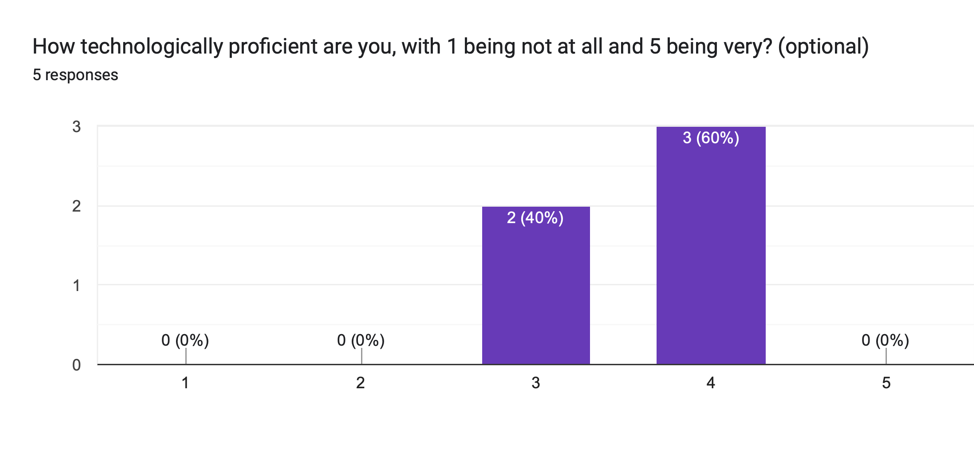
\includegraphics[scale=0.6]{images/Survey1.png}\\
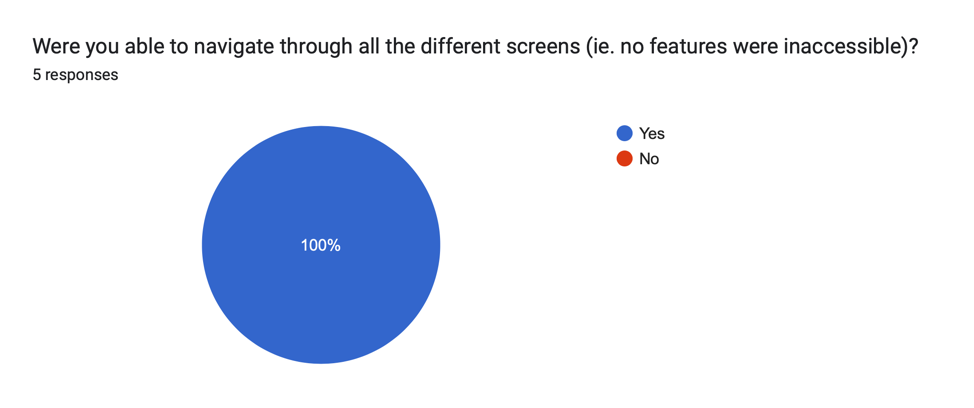
\includegraphics[scale=0.6]{images/Survey2.png}\\
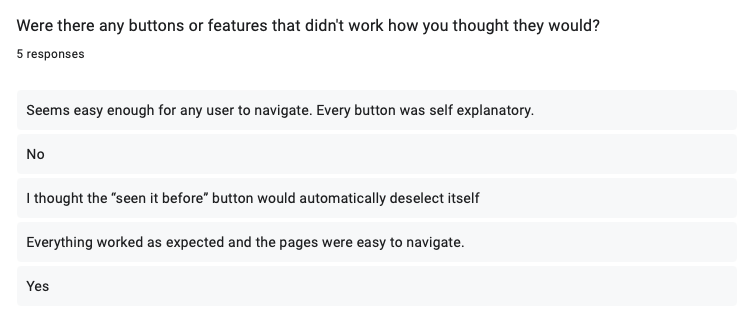
\includegraphics[scale=0.6]{images/Survey3.png}\\
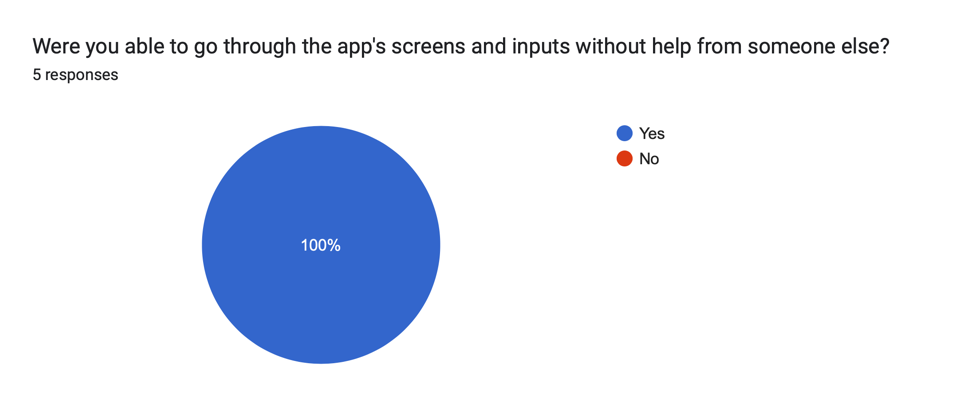
\includegraphics[scale=0.6]{images/Survey4.png}\\
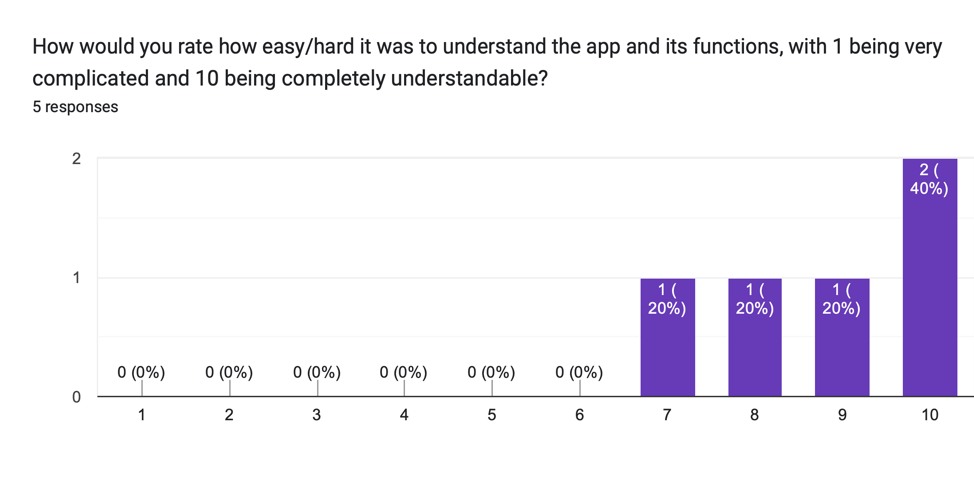
\includegraphics[scale=0.6]{images/Survey5.png}\\
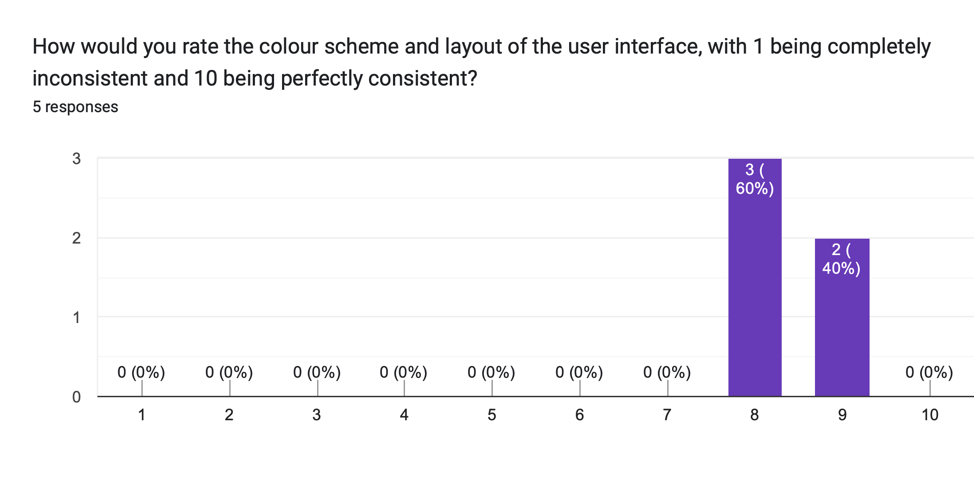
\includegraphics[scale=0.6]{images/Survey6.png}\\


\end{document}